\section{VoLTE传输协议分析}
\label{chap:backinfo:rtp}

%VoLTE实在RTP协议的基础上实现的,RTP自身有一些特征
RTP是VoLTE使用的应用层协议,通过主动丢包的方式构建时间隐通道,需要结合协议特征对数据包进行准确辨别。
%在这里进行的分析,如何利用这些特征,构造时间隐通道
在RTP协议中,存在一些固定的字段及结构,利用这些字段,不仅能够识别数据包身份,还可以提升时间隐通道的保密性。

\subsection{RTP数据包结构}
\label{chap:backinfo:rtp:struct}

%RTP是怎样的标准,数据包等层次解析
RTP以UDP作为传输层协议,不需要类似TCP的握手及挥手过程,也不会受到传输窗口的限制。因此,RTP在传输延迟及响应速度方面具有极大的优势,在实时音视频通话、互联网实时应用中得到广泛应用。\nupcite{6923336}根据数据包的组成结构,IP数据包的负载是UDP数据包内容,UDP的负载是RTP数据包内容。由于当前以太网的最大传输单元(MTU)通常设定为{1500\ Bytes},IPv6网络下IP包头长度通常为{40\ Bytes},UDP包头通常为{8\ Bytes},RTP包头通常为{12\ Bytes},所以RTP的负载数据通常不超过{1440\ Bytes}。\nupcite{6269462}因此,待发送的视频帧必须分包传输,大大增加了视频数据包的数量。

\insertFigure{
	\begin{figure}[htbp]
		\centering
        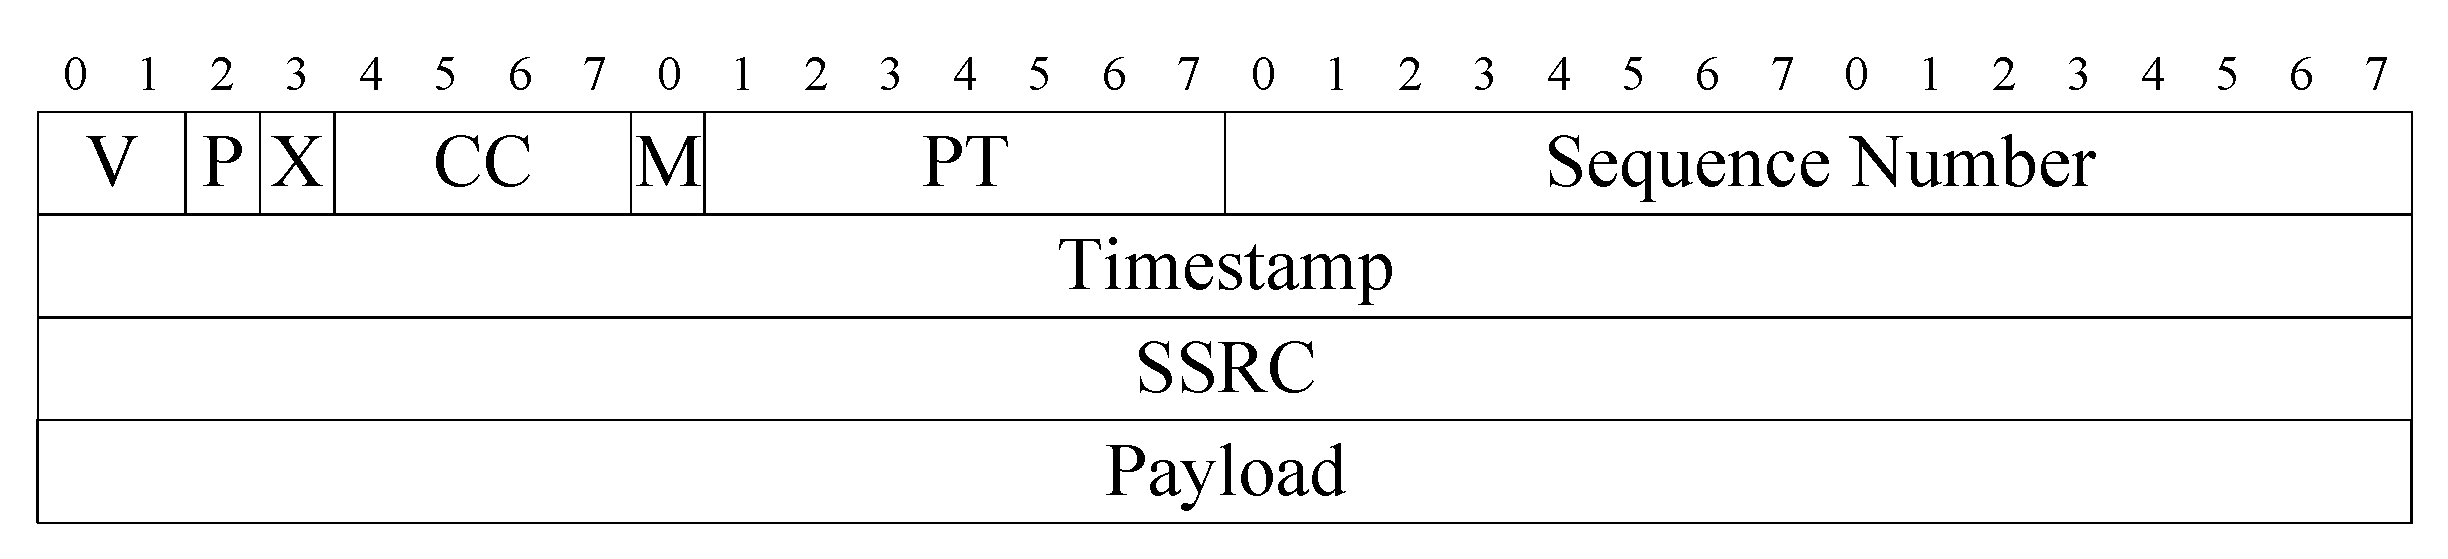
\includegraphics[width=0.9\textwidth]{chapters/chapter2/figures/rtp-header.pdf}
        \caption{RTP包头结构示意图}\label{fig:2:rtp-header}
	\end{figure}
}

%RTP头的组成
VoLTE中常用的RTP包头结构如图\nref{fig:2:rtp-header},在包头中存在固定的字段,如V({Version})表明RTP协议版本,M({Marker})指示负载分片的终止,PT({Payload Type})指明数据负载的类型。\nupcite{6923336}

\subsection{随机字段}
\label{chap:backinfo:rtp:random}

%RTP参数中,包含哪些随机生成的字段
RTP数据包头中,存在一些特殊的字段,其取值在标准中有隐含要求。

%SSRC、TimeStamp,生成的效果
图\nref{fig:2:rtp-header}中的{Sequence Number}字段,用于标识一次通话中的数据包顺序,按照步长为1的规律递增。数据包序号的初始值应该随机生成,从而抵御已知明文攻击。

图\nref{fig:2:rtp-header}中的{Timestamp}字段,反映了采样时间的变化,便于接收方在网络抖动时,按照正确的时序进行数据处理。该字段的初始值也应该为随机值,在不同的传输流中,体现了各自采样时间的变化。\nupcite{6156339}

图\nref{fig:2:rtp-header}中的{SSRC}({Synchronization Source identifier})字段,用于标记数据源。该字段取值必须随机生成,从而避免在一次RTP会话中出现相同的{SSRC},如果发生了数据源改变,该字段必须重新生成。{SSRC}字段的设计,实现了字段值与特定数据流的对应,实现了流量标识的功能。\nupcite{6222709}

%用于时间隐通道的秘钥及随机特征生成,保证保密性
时间隐通道作为隐蔽传输方法,传输的数据不应该被破解或截获。借助RTP中的这些随机字段,迭代伪随机数生成算法,为每次传输生成随机扰动,从而有效防范对隐蔽消息的破解。

\subsection{RTP丢包处理}
\label{chap:backinfo:rtp:dropout}

%RTP及应用中,对于丢包事件的处理
根据RTP数据包的层次结构,丢包影响需要综合各层次的响应。对于IP层,无法感知丢包事件,也不会出现重传行为;UDP本身不具备重传及确认机制,无法保证数据包送达,也不存在重传行为;RTP重点在于实时性,而重传会导致数据阻塞,从而破坏实时性效果,因此只在RTCP数据包中反馈网络质量。\nupcite{6423613,5478577,6894614}

%丢包不重传,序号保证自增,是主动丢包方法的基础
RTP中数据包序号不重复、丢包后不重传,是基于主动丢包时间隐通道的构建基础。对于隐通道发送方,在发送方丢弃的数据包,接收方一定可以感知到。同时数据包序号具有同步时钟的功能,时间隐通道根据序号范围分别进行丢包,即可确保数据接收总量的一致性。